\documentclass[a4paper,12pt]{article} 
\usepackage[T2A]{fontenc}			
\usepackage[utf8]{inputenc}			
\usepackage[english,russian]{babel}	
\usepackage{amsmath,amsfonts,amssymb,amsthm,mathtools} 
\usepackage[colorlinks, linkcolor = blue]{hyperref}
\usepackage{upgreek}\usepackage[left=2cm,right=2cm,top=2cm,bottom=3cm,bindingoffset=0cm]{geometry}
\usepackage{multirow}
\usepackage{graphicx}
\usepackage{xcolor}
\usepackage{multirow}

\author{Шелихов Дмитрий\\Группа Б01-305}

\title{\textbf{Работа 3.2.2\\Резонанс напряжений в последовательном контуре}} 
\date{\today}

\begin{document} 

\maketitle

\textbf{Цель работы:} исследование резонанса напряжений в последовательном колебательном контуре с изменяемой ёмкостью, получение амплитудно-частотных и фазово-частотных характеристик, определение основных параметров контура.

\textbf{В работе используются:} генератор сигналов, источник напряжения, нагрузкой которого является последовательный колебательный контур с переменной ёмкостью, двухканальный осциллограф, цифровые вольтметры.

\noindent\textbf{Экспериментальная установка}

В работе изучается резонанс напряжений в последовательном колебательном контуре (рис. 1). Напряжение $\mathcal{E}$ на контуре попадает одновременно на канал 1 осциллографа и вход 1-го цифрового вольтметра. Напряжение на конденсаторе $U_c$ подается одновременно на канал 2 осциллографа и вход 2-го цифрового вольметра.

\begin{figure}
\begin{center}
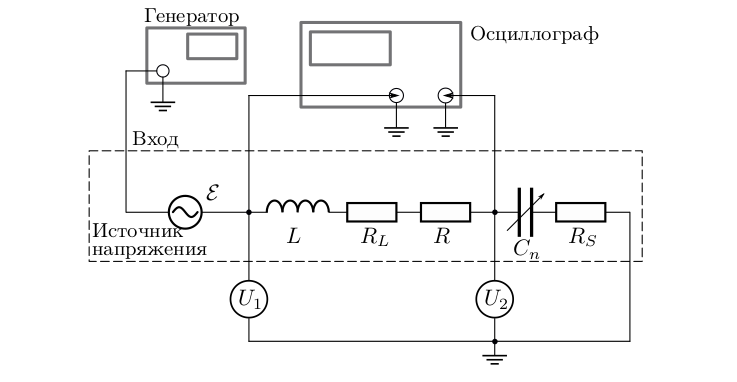
\includegraphics[width = 0.5\textwidth]{1.png}
\caption{Схема экспериментального стенда}
\end{center}
\end{figure}


\noindent\textbf{Ход работы} 

1. Настроим работу экспериментальной установки по техническому описанию. В двухканальном режиме работы осциллографа установим общее начало отсчёта $Y_1(t)$, $Y_2(t)$ вблизи левого края средней линии экрана. В качестве синхронизирующего сигнала выберем напряжение $\mathcal{E}$(t) при начальных условиях: $\mathcal{E}$(0) = 0, $\dot{\mathcal{E}}$ < 0.

2. Установим на выходе генератора эффективное значение напряжения $\mathcal{E}$ = 200 мВ. Меняя частоту $\nu$ = $\omega$/2$\pi$ генератора, убеждаемся, что у синусоиды $U_c$(t) меняется амплитуда и фаза относительно начала координат, в то время как синхронизирующий сигнал $\mathcal{E}$(t) привязан к началу отсчёта, и его амплитуда $\mathcal{E}_0$ остаётся неизменной с относительной погрешностью менее 1\%. 

3. Переключая на блоке 7 различных ёмкостей $C_n$ измерим резонансные частоты $\nu_{0n}$ и напряжения $U_C$($\nu_{0n}$) при установленном напряжении $\mathcal{E}$ на выходе генератора. Также зарегистрируем напряжения $\mathcal{E}$($\nu_{0n}$), игнорируя отклонения в пределах относительной погрешности 1\%. 

\begin{tabular}{|c|c|c|c|}
\hline
$C_n$, нФ & $f_{0n}$, кГц & $U_C$, В & $\mathcal{E}$, В \\
\hline
25,0 & 31,3 & 4,89 & 0,206 \\
33,2 & 27,3 & 4,31 & 0,206 \\
47,5 & 23,0 & 3,81 & 0,206 \\
57,2 & 21,0 & 3,54 & 0,206 \\
67,4 & 19,4 & 3,23 & 0,206 \\
82,1 & 17,5 & 3,04 & 0,206 \\
99,6 & 15,9 & 2,81 & 0,206 \\
\hline
\end{tabular}

4. Проделаем измерения п.3 для входного напряжения $\mathcal{E}$ = 0,4 мВ 

\begin{tabular}{|c|c|c|c|}
\hline
$C_n$, нФ & $f_{0n}$, кГц & $U_C$, В & $\mathcal{E}$, В \\
\hline
25,0 & 31,2 & 9,28 & 0,4 \\
33,2 & 27,2 & 6,16 & 0,4 \\
47,5 & 22,9 & 7,31 & 0,4 \\
57,2 & 20,9 & 6,79 & 0,4 \\
67,4 & 19,3 & 6,32 & 0,4 \\
82,1 & 17,5 & 5,65 & 0,4 \\
99,6 & 15,9 & 5,40 & 0,4 \\
\hline
\end{tabular}

5. Для контуров с ёмкостями $C_{n1}$ = 25,0 нФ и $C_{n7}$ = 99,6 нФ измерим амплитудно-частотные характеристики $U_C$($\nu$) для значений $U_C$($\nu$) $\geq$ 0,6$U_C$($\nu_{0n}$) 

\begin{tabular}{|c|c|c|}
\hline
$C_{n1}$, нФ & $\nu$, кГц & $U_C$($\nu$), В \\
\hline
\multirow{20}{*}{25,0} & 30,56 & 3,00 \\
\cline{2-3} & 30,66 & 3,28 \\
\cline{2-3} & 30,76 & 3,58 \\
\cline{2-3} & 30,86 & 3,93 \\
\cline{2-3} & 30,96 & 4,27 \\
\cline{2-3} & 31,06 & 4,58 \\
\cline{2-3} & 31,16 & 4,81 \\
\cline{2-3} & 31,26 & 4,93 \\
\cline{2-3} & 31,36 & 4,93 \\
\cline{2-3} & 31,46 & 4,81 \\
\cline{2-3} & 31,56 & 4,61 \\
\cline{2-3} & 31,66 & 4,39 \\
\cline{2-3} & 31,76 & 4,12 \\
\cline{2-3} & 31,86 & 3,87 \\
\cline{2-3} & 31,96 & 3,61 \\
\cline{2-3} & 32,06 & 3,38 \\
\cline{2-3} & 32,16 & 3,15 \\
\cline{2-3} & 32,26 & 2,95 \\
\cline{2-3} & 32,36 & 2,76 \\
\cline{2-3} & 32,46 & 2,58 \\
\hline
\end{tabular}
\qquad
\begin{tabular}{|c|c|c|}
\hline
$C_{n7}$, нФ & $\nu$, кГц & $U_C$($\nu$), В \\
\hline
\multirow{17}{*}{99,6} & 15,24 & 1,71 \\
\cline{2-3} & 15,34 & 1,87 \\
\cline{2-3} & 15,44 & 2,06 \\
\cline{2-3} & 15,54 & 2,26 \\
\cline{2-3} & 15,64 & 2,46 \\
\cline{2-3} & 15,74 & 2,65 \\
\cline{2-3} & 15,84 & 2,78 \\
\cline{2-3} & 15,94 & 2,84 \\
\cline{2-3} & 16,04 & 2,80 \\
\cline{2-3} & 16,14 & 2,69 \\
\cline{2-3} & 16,24 & 2,54 \\
\cline{2-3} & 16,34 & 2,36 \\
\cline{2-3} & 16,44 & 2,18 \\
\cline{2-3} & 16,54 & 2,01 \\
\cline{2-3} & 16,64 & 1,85 \\
\cline{2-3} & 16,74 & 1,70 \\
\cline{2-3} & 16,84 & 1,57 \\
\hline
\end{tabular}

6. Для тех же двух контуров измерим фазо-частотную характеристику $\psi_C$($\nu$) для значений $U_C$($\nu$) $\geq$ 0,3$U_C$($\nu_{0n}$) при том же значении $\mathcal(E)$, что и в п.3 (0,2 В) 

$$\Delta\varphi = \frac x{x_0}\pi$$

\begin{tabular}{|c|c|c|c|c|}
\hline
$C_{n1}$, нФ & $\nu$, кГц & x($\nu$), дел & $x_0$, дел & $\Delta$$\phi$, рад\\
\hline
\multirow{12}{*}{25,0} & 29,75 & 2 & \multirow{12}{*}{17} & 0,37\\
\cline{2-3} & 30,45 & 3 & & 0,55\\
\cline{2-3} & 30,70 & 4 & & 0,74\\
\cline{2-3} & 30,89 & 5 & & 0,92\\
\cline{2-3} & 31,03 & 6 & & 1,11\\
\cline{2-3} & 31,16 & 7 & & 1,29\\
\cline{2-3} & 31,29 & 8 & & 1,48\\
\cline{2-3} & 31,41 & 9 & & 1,66\\
\cline{2-3} & 31,58 & 10 & & 1,85\\
\cline{2-3} & 31,75 & 11 & & 2,03\\
\cline{2-3} & 32,02 & 12 & & 2,22\\
\cline{2-3} & 32,44 & 13 & & 2,40\\
\hline
\end{tabular}
\qquad








\end{document}
